\documentclass[10pt,a4paper]{report}
\usepackage[utf8]{inputenc}
\usepackage{amsmath}
\usepackage{amsfonts}
\usepackage{amssymb}
\usepackage{fancyhdr}
\usepackage{tikz}

\usetikzlibrary{positioning, arrows, backgrounds, fit}
\usepackage{titlesec, blindtext, color}
\newcommand{\hsp}{\hspace{20pt}}
\titleformat{\chapter}[hang]{\Huge\bfseries}{\thechapter\hsp}{0pt}{\Huge\bfseries}

\begin{document}
\chapter{Augmented Chess:\\ Assignment 4}

\begin{center}
{\Large \textbf{Group Members}}

\begin{tabular}{l r}
Jacob Holm Mortensen		&	jmorte14@student.aau.dk\\
Martin Raunkjær Andersen	&	marand13@student.aau.dk\\
Thomas Gwynfryn McCollin	&	tmccol14@student.aau.dk
\end{tabular}
\end{center}

\section{Adaptations}
This section will discuss the current and planned adaptations in the web application. The web application is personalised, but does not treat audiences from different regions differently. Therefore the focus of this section will be explaining the personalization and discussing the possible localisation and internationalisation for the application.

\subsection{Personalisation}
Users may register themselves under any user-name and begin creating armies and playing the game. Any army which is created by the user can be stored for later use. Furthermore any game related statistics are recorded and associated with that user-name. Further personalisation is possible, but is not planned at the moment.

\subsection{Localisation and Internationalisation}
The application will not differentiate users, however this could be implemented in a hypothetical future version. Chess is played in most countries so it reasonable to assume non-English speaking player would like to play Augmented Chess. Therefore translation of the application could be performed at page generation. Chess uses the same notation everywhere so unit translation is unnecessary. Finally data format and statistical representation could be accounted for. An example of this is the number ten thousand is written as 10,000 in English, however it is written 10.000 in Danish. 

\section{Design Patterns}
The application is written in Angular 2, which is set up to use the Model View Controller (MVC) design pattern. So far in development we have used this pattern however we will likely switch to the Model View ViewModel (MVVM). The advantage of MVVM over MVC is that the View and ViewModel are properly separated in MVVM, while in MVC changes in the View will probably warrant changes in the Controller. This is not the case in MVVM, since the ViewModel consists of triggers and bindings any changes in the View will most likely not require changes in the ViewModel.

\section{Implementation}
The application is implemented based on the design specified earlier in this course. The design concerns it self primarily with the data model, which represents data in the application, and the site view, which represents pages and navigation between them.

\subsection{Data}
\begin{minipage}{.35\textwidth}
The data in the application primarily consists of armies and pieces. These are sent back forth between the client and server via services. These services serve as an interface to the database. Data is passed as JSON objects through the services. Synchronisation is handled locally by the service and the database ensures server-side synchronisation.
\end{minipage}
\hfill
\begin{minipage}{.55\textwidth}

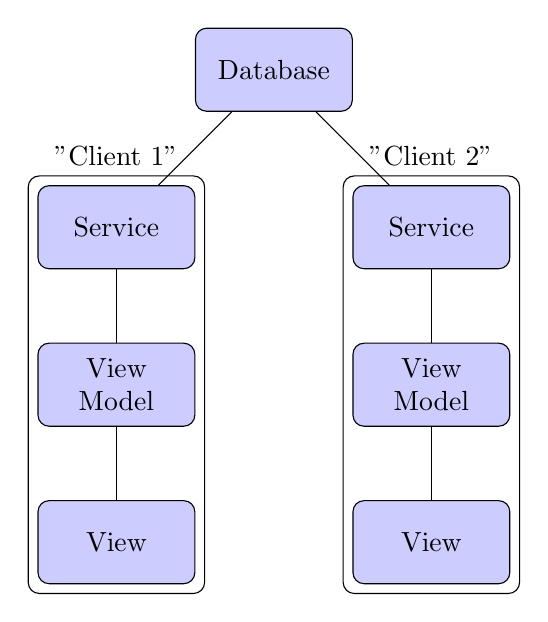
\begin{tikzpicture}
\tikzstyle{block}=[draw, rectangle, fill=blue!20, rounded corners, text centered, minimum height = 3em, text width = 5em]

\node[block](db) at (0,0){Database};

\node[block](serv1) 	at	(-2,-2){Service};
\node[block](vm1) 		at	(-2,-4){View Model};
\node[block](view1) 		at	(-2,-6){View};

\node[block](serv2) 	at	(2,-2){Service};
\node[block](vm2) 		at	(2,-4){View Model};
\node[block](view2) 	at	(2,-6){View};

\path[draw](serv1) -- (db);
\path[draw](vm1) -- (serv1);
\path[draw](view1) -- (vm1);

\path[draw](serv2) -- (db);
\path[draw](vm2) -- (serv2);
\path[draw](view2) -- (vm2);

\node[fit=(serv1) (vm1) (view1), rectangle, rounded corners, draw, label="Client 1"]{};
\node[fit=(serv2) (vm2) (view2), rectangle, rounded corners, draw, label="Client 2"]{};

\end{tikzpicture}
\end{minipage}

\subsection{Navigation and Pages}
The pages and links from the site view of our design translate directly into components and routes in angular 2. Each page has a component, which consists of view and viewmodel and may be connected to a service. The view is pure \texttt{HTML/CSS} and the logic is \texttt{TypeScript}, which is a strongly typed variation of \texttt{JavaScript}. The logic is further extended by the angular 2 framework. Pages are linked together via routing which is simply the angular 2 flavour of links. Minor changes have occured in relation to the data as we encounter requirements we had foreseen however the pages and links between them has been closely consistent with the design. 


\end{document}